\chapterimage{ChapterImageLaboratory.png} % Chapter heading image

\chapter{Wastewater Laboratory Analysis}

% \section{Paragraphs of Text}\index{Paragraphs of Text}


% \everymath{\displaystyle}
% \linespread{2}%controls the spacing between lines. Bigger fractions means crowded lines%
% %\pagestyle{fancy}
% %\usepackage[margin=1 in, top=1in, includefoot]{geometry}
% %\everymath{\displaystyle}
% \linespread{2}%controls the spacing between lines. Bigger fractions means crowded lines%
% %\pagestyle{fancy}
% \pagestyle{fancy}
% \setlength{\headheight}{56.2pt}
% \colorlet{Mycolor1}{green!10!orange!90!}

% \chead{\ifthenelse{\value{page}=1}{
\includegraphics[scale=0.3]{SCC}\\ \textbf \textbf Introduction to Wastewater Treatment}}
% \rhead{\ifthenelse{\value{page}=1}{}{}}
% \lhead{\ifthenelse{\value{page}=1}{}{\textbf Introduction to Wastewater Treatment}}
% \rfoot{\ifthenelse{\value{page}=1}{Module 1: WATR 048 - Spring 2019}{Module 1: WATR 048 - Spring 2019}}

% \cfoot{Page \thepage\ of \pageref{LastPage}}
% \lfoot{Shabbir Basrai}
% \renewcommand{\headrulewidth}{2pt}
% \renewcommand{\footrulewidth}{1pt}

% \newcommand{\stkout}[1]{\ifmmode\text{\sout{\ensuremath{#1}}}\else\sout{#1}\fi}
% %Defining colour with different models.
% \definecolor{mypink1}{rgb}{0.858, 0.188, 0.478}
% \definecolor{mypink2}{RGB}{219, 48, 122}
% \definecolor{mypink3}{cmyk}{0, 0.7808, 0.4429, 0.1412}
% \definecolor{mygray}{gray}{0.6}
% \colorlet{LightRubineRed}{RubineRed!70!}
% \colorlet{Mycolor1}{green!10!orange!90!}
% \definecolor{Mycolor2}{HTML}{00F9DE}

% %New command used in the table with all available colour names
% \newcommand{\thiscolor}[1]{\texttt{#1} \hfill \fcolorbox{black}{#1}{\hspace{2mm}}}

% %This changes the row separation in the table
% \renewcommand{\arraystretch}{1.5}




%\noindent\textsc{Area \& Volume Math Problems}
%\definecolor{shadecolor}{RGB}{200,200,240}
% \item \noindent\textsc{Why Treat Wastewater}


		\section{BOD Analysis}\index{BOD Analysis}		
\begin{itemize}
\setlength\itemsep{1em}

\item The Biochemical Oxygen Demand (BOD) test estimates the amount of biodegradable material present by measuring the amount of oxygen used by the bacteria to break down the organic waste in the sample incubated at 20 deg. C over a five-day period . The BOD test provides an indication on the strength of wastewater in terms of how much oxygen could be depleted if that wastewater was introduced into another receiving water.  Complete stabilization of a sample may require a period of incubation too long for practical purposes; therefore, 5 days has been accepted as the standard incubation period.

\item As the regular BOD test includes estimation of oxygen nitrifying bacteria consumes in the process of converting inorganic forms of ammonia and nitrogen to nitrite and nitrate, its value represents oxygen used for removing both, organic material and nitrogenous matter.  As this BOD value does not quite represent the organic strength of the wastewater, the normal BOD test is modified by introducing a chemical inhibitor - 3 mg of 2-chloro-6-(trichloro methyl) pyridine (TCMP), which suppresses the growth of the nitrogenous bacteria so that the resultant BOD measured represents the oxygen depletion associated with the depletion of the organic matter only.  This is the Carbonaceous biochemical oxygen demand or cBOD. \\
\vspace{0.4cm}
\textbf{Thus tBOD = nBOD + cBOD}

\item Wastewater BOD measurement involves testing a sample set consisting of several sample dilutions along with a "Blank".  "Blank" is a sample with only the dilution water with no wastewater added. \\

\vspace{0.4cm}



\item The dilutions are made based upon the expected BOD concentration of the sample.  Using the final dilution volume of 300 ml, the initial sample volume can be estimated using the formula:\\
\vspace{0.4cm}

\textbf{$Sample \enspace Volume (ml) = \dfrac{\Big[Oxygen \enspace Depletion \Big(\dfrac{mg}{l}\Big)\Big]}{Anticipated \enspace BOD \Big(\dfrac{mg}{l}\Big)}*300 \enspace ml$}\\

\vspace{0.4cm}
\item For example, if testing an influent wastewater BOD with an expected BOD value of 250 mg/l, a range of sample volumes for dilution around sample volume of $\dfrac{4\dfrac{mg}{l}}{250 \dfrac{mg}{l}}*300 \enspace ml$=5ml.\\
\vspace{0.4cm}
\item The data obtained for each of the dilutions after the 5-day incubation period must meet the following criteria for the sample value to be acceptable for calculating the BOD.\\
\vspace{0.4cm}

\begin{enumerate}[1.]
\setlength\itemsep{1em}

\item A residual DO of at least 1 mg/L,
\item A DO depletion of at least 2 mg/L
\end{enumerate}
\vspace{0.4cm}
\item Additionally, the whole sample set is rejected if the Blank shows an oxygen depletion of >0.2mg/l.\\
\vspace{0.4cm}
\item BOD is calculated for each sample dilution value using the following formula:\\
\vspace{0.4cm}
\textbf{$BOD \Big(\dfrac{mg}{l}\Big) = \dfrac{Initial \enspace DO - DO \enspace Day \enspace 5}{Sample \enspace Volume \enspace (ml)}*300 \enspace ml$}\\



\end{itemize}
\vspace{0.4cm}
\section{Wastewater solids}\index{Wastewater solids}

	\subsection{Total (TSS) and Volatile (VSS)}\index{Total (TSS) and Volatile (VSS)}
\begin{itemize}
\setlength\itemsep{1em}
					\item A known volume of wastewater sample is filtered through a pre-weighed filter paper
					\item The suspended solids will be retained by the filter
					\item The water with the dissolved solids will pass through the filter
					\item The filter paper with the filter solids is rinsed with distilled water to remove 
					\item The filter paper with the solids is dried in the oven and then weighed
					\item The difference between the weight of the dried filter paper with the solids and the pre-weighed filter paper, measured in mg, will be the suspended solids in: mg per the original quantity of wastewater sample taken.  This value can be converted to give the suspended solids content in mg/l
					\item A filter paper with the dried solids is incinerated in a muffler furnace
					\item The difference in the weight of the solids, before and after incineration is the fixed solids
					\item The difference between the weight of the solids before incineration and the fixed solids is the volatile solids
	\end{itemize}				

\textbf{Total Suspended Solids - TSS}
\vspace{0.4cm}
$TSS \dfrac{mg}{l}=\dfrac{weight \enspace of \enspace solids \enspace \cancel{gms}}{volume \enspace of \enspace sample \enspace \enspace \cancel{ml}}*\dfrac{1000 \enspace \cancel{ml}}{l}*\dfrac{1000 \enspace mg}{\cancel{gms}}$\\
\vspace{0.3cm}
\hspace{1.4cm}$=\dfrac{weight \enspace of \enspace filter \enspace paper  \enspace with \enspace dried  \enspace solids - weight \enspace of \enspace filter \enspace paper}{volume \enspace of \enspace sample \enspace \enspace (ml)}*1,000,000$\\
\vspace{0.4cm}

\vspace{0.4cm}
\textbf{Volatile Suspended Solids - VSS}	
\vspace{0.4cm}

$VSS \dfrac{mg}{l}=\dfrac{weight \enspace of \enspace volatile \enspace solids \enspace \cancel{gms}}{volume \enspace of \enspace sample \enspace \enspace \cancel{ml}}*\dfrac{1000 \enspace \cancel{ml}}{l}*\dfrac{1000 \enspace mg}{\cancel{gms}}$\\
\vspace{0.3cm}
\hspace{1.4cm}$=\dfrac{wt. \enspace of \enspace filter \enspace paper  \enspace with \enspace dried  \enspace solids - wt. \enspace of \enspace filter \enspace paper \enspace incinerated \enspace residue}{volume \enspace of \enspace sample \enspace \enspace (ml)}*1,000,000$\\
\vspace{0.3cm}
$VSS(\%)=\dfrac{weight \enspace (gms) \enspace of \enspace volatile \enspace solids}{100 \enspace gms \enspace total \enspace solids}=\dfrac{gms \enspace volatile \enspace solids}{\cancel{gms \enspace total \enspace solids}}*\dfrac{100 \cancel{\enspace gms \enspace total \enspace solids}}{100 \enspace gms \enspace total \enspace solids}$\\
\vspace{0.3cm}
\hspace{1.5cm}\small{$=\dfrac{wt. \enspace of \enspace filter \enspace paper  \enspace with \enspace dried  \enspace solids - wt. \enspace of \enspace filter \enspace paper \enspace incinerated \enspace residue}{wt. \enspace of \enspace filter \enspace paper  \enspace with \enspace dried  \enspace solids - wt. \enspace of \enspace filter \enspace paper}*100$}\\				

	\subsection{Wastewater and Sludge Total \& Volatile Solids}\index{Wastewater and Sludge Total \& Volatile Solids}
\vspace{0.4cm}
\begin{itemize}
\setlength\itemsep{1em}
					\item A certain quantity of wastewater (by volume) or sludge (by weight) is taken in a pre-weighed dish and weighed.  \hl{Note:  the sample is not filtered.}
					\item The dish with the sample is dried in an oven
					\item The difference in the weight of the pre-weighed dish from that of the dish with the dried sample is the total solids
					\item The dried solids are incinerated in a muffler furnace
					\item The difference in the weight of the solids, before and after incineration is the fixed solids
					\item The difference between the fixed solids and the total solids is the volatile solids
					\item Total solids of a sludge sample is reported as a \% of the sludge weight.  A 7\% sludge has 7 lbs of solids for every 100 lbs of sludge.
				\end{itemize}
				
				\hl{For sludge samples, volatile solids is typically reported as the volatile solids fraction in \% of the total solids content of the sludge.  For example, if a 8\% sludge (i.e sludge which has 8\% TS or 80,000mg/l solids), is reported to have 70\% volatile, it means that 70\% of the total solids - 0.7*8\%=5.6\% or 56,000mg/l is the sludge volatile solids content.  \emph{70\% volatile does not meet the sludge has 700,000mg/l volatile solids}}\\	

\vspace{0.4cm}
\textbf{Total Solids - TS}			
\vspace{0.4cm}
$TS(\%)=\dfrac{weight \enspace of \enspace solids \enspace (gms)}{100 \enspace gms \enspace of \enspace sample}=\dfrac{gms \enspace solids}{gms \enspace sample}*100$\\
\vspace{0.3cm}
\hspace{1.2cm}$=\dfrac{weight \enspace of \enspace cruicible \enspace with \enspace dried  \enspace solids - weight \enspace of cruicible}{weight \enspace of \enspace cruicible \enspace with \enspace sample - weight \enspace of cruicible}*100$\\
\vspace{0.4cm}
\textbf{Total Volatile Solids - VS}		
\vspace{0.4cm}
$VS(\%)=\dfrac{weight \enspace of \enspace volatile \enspace solids \enspace (gms)}{100 \enspace gms \enspace of \enspace total \enspace solids}=\dfrac{gms \enspace volatile \enspace solids}{gms \enspace total \enspace solids}*100$\\
\vspace{0.3cm}
\hspace{1.2cm}$=\dfrac{wt. \enspace of \enspace cruicible  \enspace with \enspace dried  \enspace solids - wt. \enspace of \enspace cruicible \enspace incinerated \enspace residue}{wt. \enspace of \enspace cruicible  \enspace with \enspace dried  \enspace solids - wt. \enspace of \enspace cruicible}*100$\\
				\newpage
				\thispagestyle{empty}
				\begin{sidewaysfigure}
					\begin{center}
						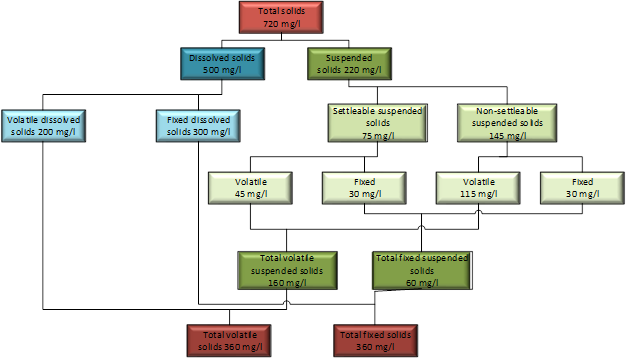
\includegraphics[scale=1.1]{WastewaterSolids}\\
						\caption{Typical Wastewater Solids Concentrations}
					\end{center}
				\end{sidewaysfigure}
\newpage
\thispagestyle{empty}
% \begin{landscape}
% \begin{center}
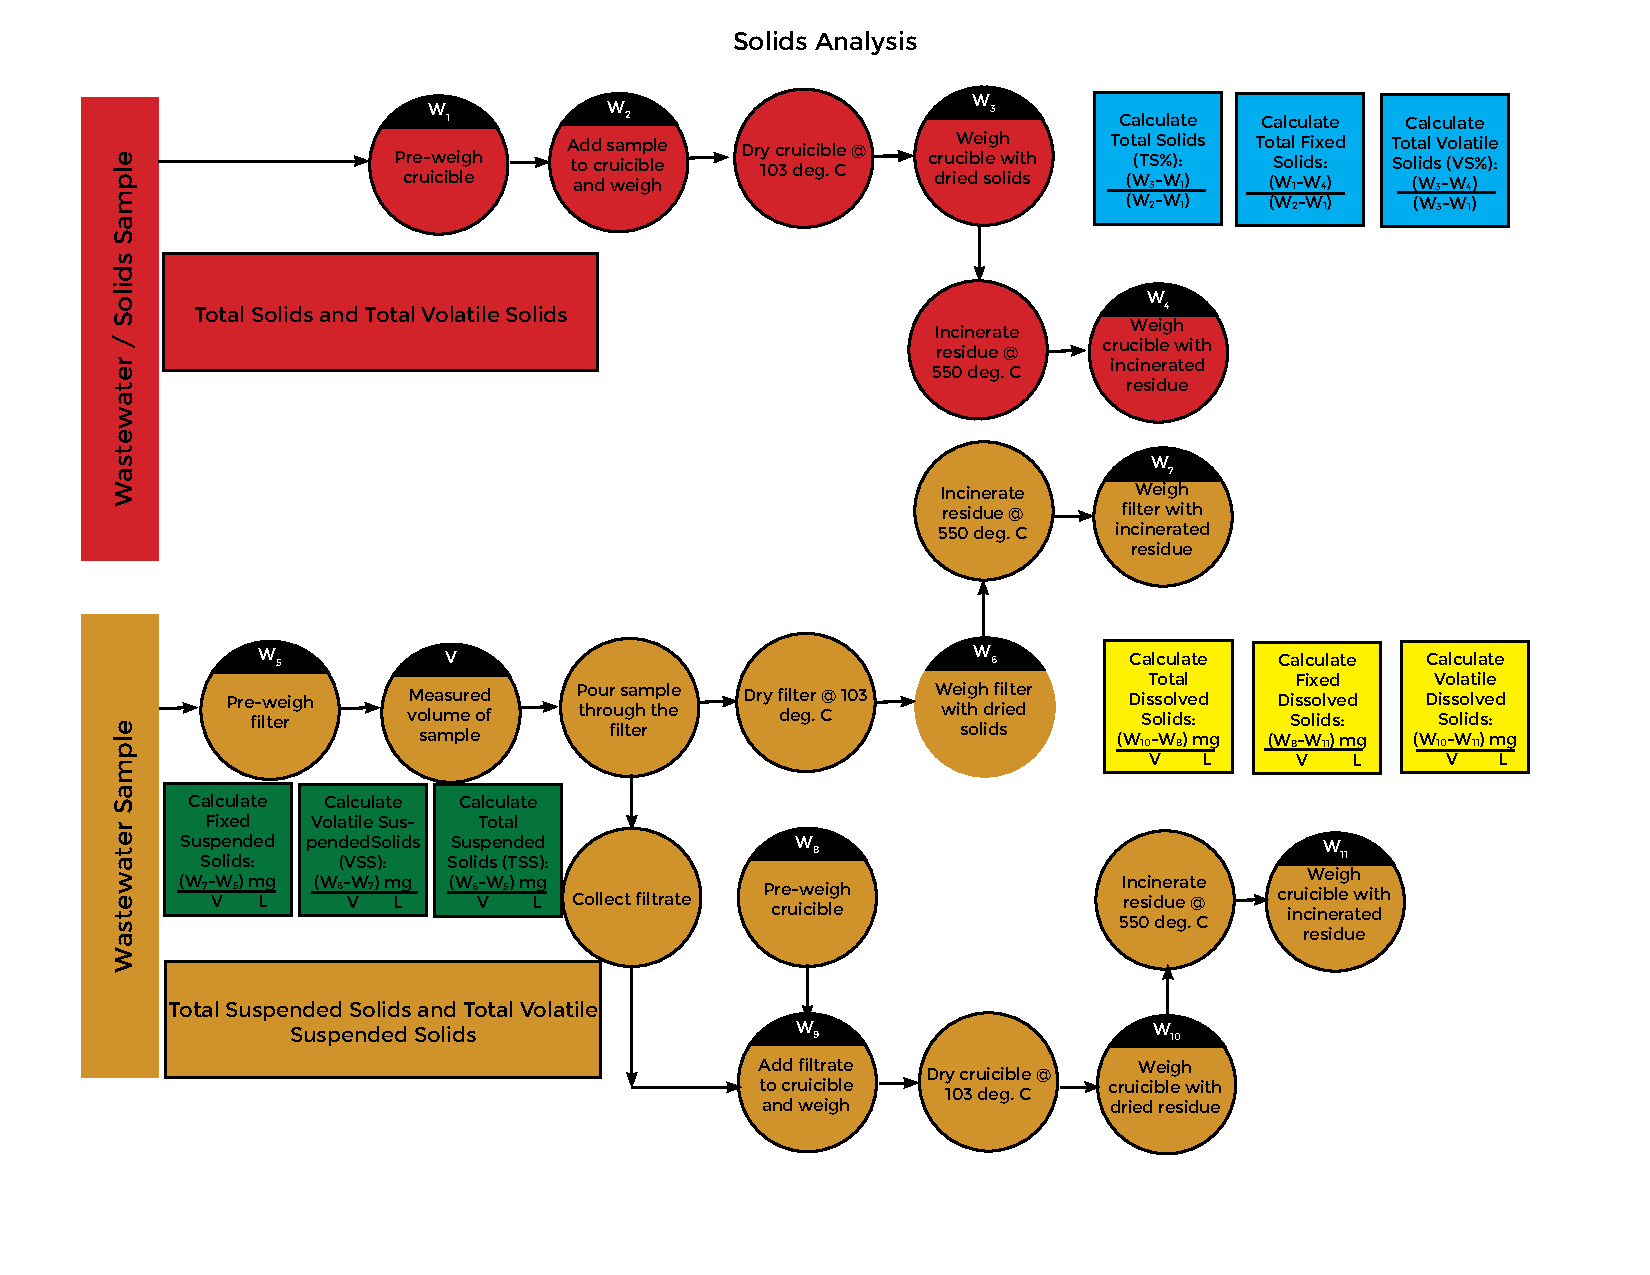
\includepdf[landscape=true]{LaboratorySolidsAnalysis4_01.pdf}
%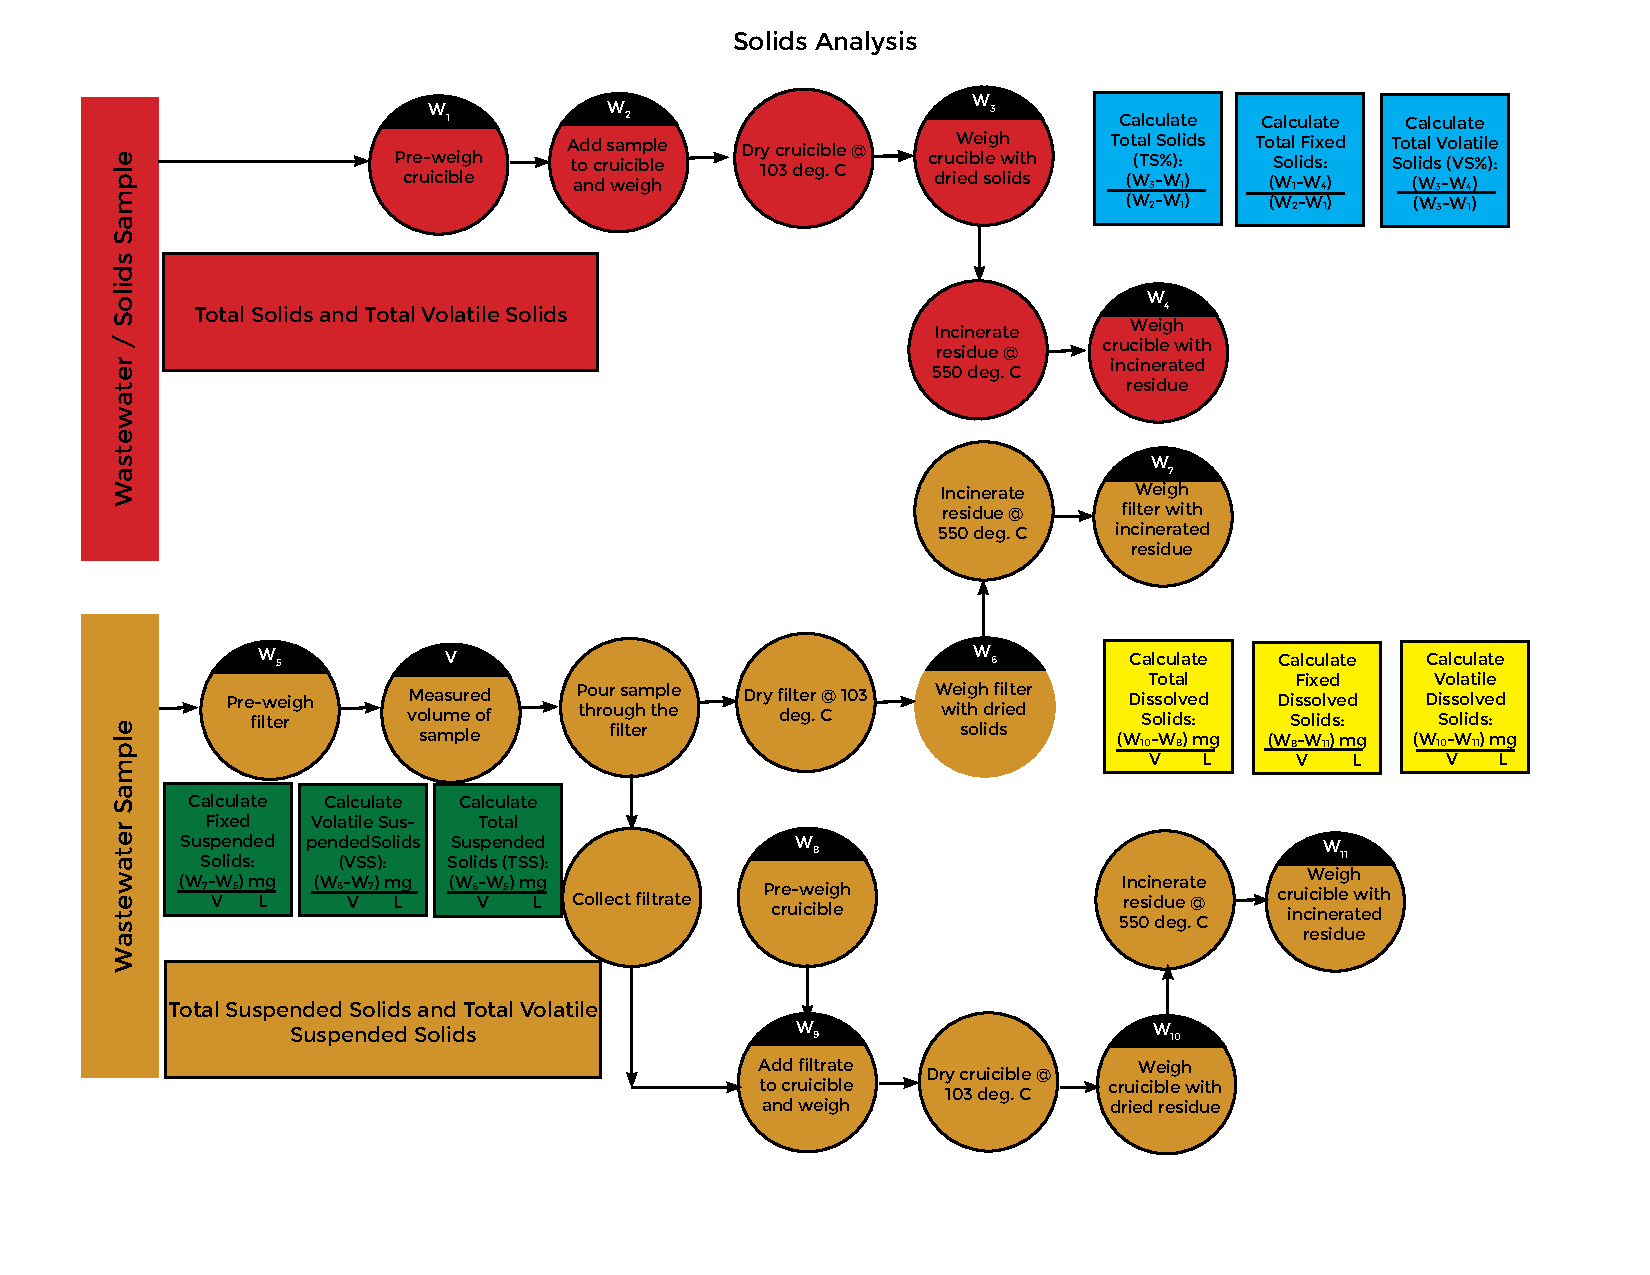
\includegraphics[scale=0.69]{LaboratorySolidsAnalysis4_01.pdf}
% \end{center}
% \end{landscape}
\subsection{Sample BOD and solids analysis math problems}\index{Sample BOD and solids analysis math problems}
\begin{enumerate}
\item BOD tests are run on the final effluent from an activated sludge plant with and without the use of a "nitrification inhibitor". Three hundred milliliter bottles (300 ml) are used in these tests. The raw data for these tests are presented below.  What \textbf{percentage of the average total BOD is the average nBOD}?\\
\vspace{0.5cm}
\begin{tabular}{m {4 cm} m {1.5 cm} m  {1.5 cm} m  {1.5 cm} m  {1.5 cm} m {1.5 cm}}
\cline{1-6}
Sample Volume, ml    & 10 & 20 & 30 & 40 & Blank\\
\hline
Initial DO, mg/l 			& 9.0 	& 	8.9 & 8.8  & 9.1 & 9.1\\
Final DO, mg/l 			& 6.9 	& 	4.8 & 2.5 & 1.1 & 9.0
\end{tabular}
\vspace{0.7cm}\\
BOD Test with "inhibitor" added	(cBOD)\\
\vspace{0.5cm}
\begin{tabular}{m {4 cm} m {1.5 cm} m  {1.5 cm} m  {1.5 cm} m  {1.5 cm} m {1.5 cm}}
\cline{1-6}
Sample Volume, ml    & 10 & 20 & 30 & 40 & Blank\\
\hline
Initial DO, mg/l 			& 8.9 	& 	8.9 & 9.0  & 9.0 & 9.1\\
Final DO, mg/l 			& 7.5 	& 	6.2 & 5.0 & 3.3 & 9.0
\end{tabular}
\vspace{0.5cm}\\
Solution:\\
Blanks for both tBOD and cBOD are both <=0.2mg/l - thus sample sets are acceptable\\
\vspace{0.5cm}
\begin{tabular}{m {3 cm} m {2.5 cm} m  {2.5 cm} m  {2.5 cm} m  {2.5 cm} }
\cline{1-5}
Sample Volume, ml    & 10 & 20 & 30 & 40 \\
\hline
tBOD Diff., mg/l    & 2.1 & 4.1 & 6.3 & 8 \\
tBOD, mg/l    & 2.1*300/10 & 4.1*300/20 & 6.3*300/30 & 8.0*300/40\\
    & =63.0 & = 61.5  & = 63.0 & = 60.0 \\
\hline
cBOD Diff., mg/l    & 1.4 & 2.7 & 4.0 & 5.7 \\
cBOD, mg/l    & Reject & 2.7*300/20 & 4.0*300/30 & 5.7*300/40\\
    & Depletion < 2 & = 40.5  & = 40 & = 42.75 \\
\end{tabular}
\vspace{0.5cm}\\

$tBOD (avg) = (63+61.5+63+60)/4=61.9 \hspace{1cm} cBOD (avg) = (40.5+40+42.75)/3=41.1$\\
nBOD = tBOD - cBOD $\implies$ nBOD = 61.9-41.1=20.8 $\implies$ nBOD(\%)=20.8/61.9*100=$\boxed{33.6\%}$
\vspace{0.5cm}
\item Calculate percent total solids and percent volatile solids of a sludge sample given the following data:\\
\begin{tabular}{m {5 cm} m {0.5 cm} m  {3.5 cm}}
Weight of dish &=&  104.55 gms\\
Weight of dish and wet sludge &= & 199.95 gms\\
Weight of dish and dry sludge &= & 108.34 gms\\
Weight of dish and ash &= & 106.37 gms
\end{tabular}\\
\vspace{0.2cm}
Solution:\\
\vspace{0.2cm}
Weight of dish=104.55 gms\\
Weight of dish and wet sludge=199.95 gms\\
Weight of dish and ash = 106.37 gms\\
\vspace{0.2cm}
$ \implies Weight \enspace of \enspace sludge=199.95-104.55=95.40 \enspace gms$\\
$\implies Weight \enspace of \enspace dry \enspace sludge \enspace (solids)=108.34-104.55=3.79 \enspace gms$\\
$\implies Weight \enspace of \enspace volatile \enspace solids=108.34-106.37=1.97 \enspace gms$\\
\vspace{0.2cm}
$Total \enspace solids (TS\%)=\dfrac{gms \enspace solids}{100 \enspace gms \enspace sludge}=\dfrac{3.79}{95.40} \enspace \dfrac{gms \enspace solids}{\cancel{gms \enspace sludge}}*\dfrac{100 \cancel{\enspace gms \enspace sludge}}{100 \enspace gms \enspace sludge}=\boxed{3.97\%}$\\
\vspace{0.2cm}
$Total \enspace volatile \enspace solids (VS\%) =\dfrac{1.97}{3.79} \enspace \dfrac{gms \enspace volatile \enspace solids}{\cancel{gms \enspace total \enspace solids}}*\dfrac{100 \cancel{\enspace gms \enspace total \enspace solids}}{100 \enspace gms \enspace total \enspace solids}=\boxed{52.0\%}$\\


\end{enumerate}

\section{Bacteriological Ennumeration}\index{Bacteriological Ennumeration}
\begin{itemize}
	\item Involves bacteriological testing of the wastewater effluent and the surface water impacted by the wastewater discharge
	
	\item Conducted in-order to:
		\begin{enumerate}
			\item Meet the requirements of a wastewater discharge permit
			\item Monitor the pathogen impact of treated wastewater discharge
			\item Assess the level of contamination of a public body of water
			\item Bacteriological tests involves detection and quantification of one or more of the following bacteria:  total coliforms, fecal coliforms, \textit{E. Coli}, and \textit{Enterococci}. 
\begin{center}
\tcbox{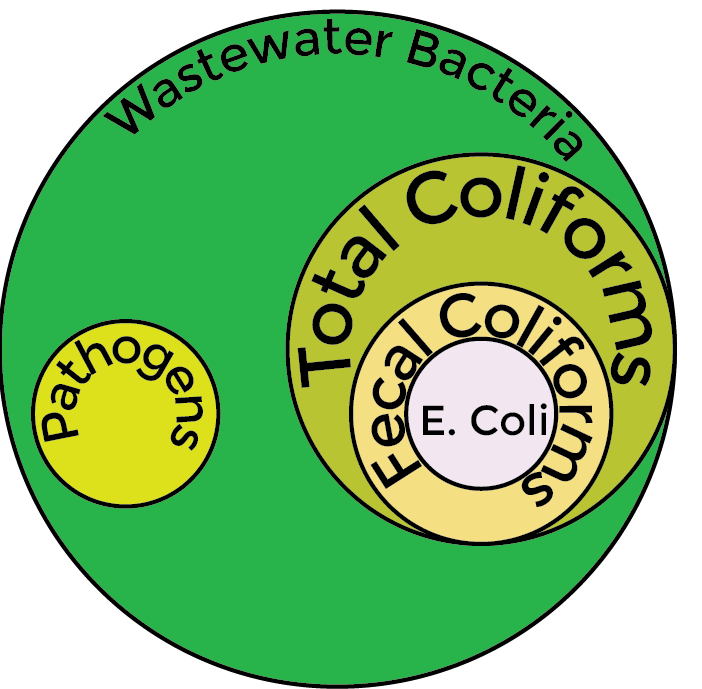
\includegraphics[width=5cm]{LaboratoryWastewaterBacteria}}
Wastewater Bacteria
\end{center}
	
	\item  In wastewater, fecal coliforms originate in the intestines of warm-blooded animals.  Aerobic bacteria including coliforms partake in the metabolization of the organic matter as part of the secondary treatment process
\item Fecal coliforms are seldom pathogenic under normal circumstances and are easily cultured, their presence indicates the potential presence of pathogens

The reason why these bacteria such as coliforms and enterococcus are used:
		\begin{enumerate}
			\item It is not practical to detect and quantify all pathogens associated with wastewater
			\item These bacteria originate from feces and indicate fecal contamination and thus serve as an indicator organisms for pathogens of wastewater origin
			\item They are also:
				\begin{itemize}
					\item abundant
					\item potentially less harmful, and
					\item easy to detect
				\end{itemize}
			\item \textit{E. coli} has been shown to be a better predictor of the potential for impacts to human health and therefore many newer wastewater discharge permits require \textit{E. Coli} testing in lieu of fecal coliform testing requirements.
		\end{enumerate}
		\end{enumerate}

\end{itemize}
 

\subsection{Bacteriological Testing Methods}\index{Bacteriological Testing Methods}
The methods for wastewater bacteriological tests include:  multiple-tube fermentation (MTF) technique, membrane filtration (MF) and quanti-tray testing.  When using the MTF and MF methods, it is not possible to exactly quantify the number of bacteria present, a statistical based - Most Probable Number (MPN) approach is utilized\\
\subsection{The Multiple-Tube Fermentation (MTF) technique}\index{The Multiple-Tube Fermentation (MTF) technique}
This involves adding three volumes – 10 ml, 1 ml and 0.1 ml of the sample, each to a set of five tubes containing Lauryl Tryptose broth and an inverted tube (Durham tube), followed by incubating the tubes at  for a specified time.  The Lauryl Tryptose broth produces color and/or turbidity change due to the growth of the target bacteria and the inverted tube collects the gas produced by the bacterial respiration.  At the end of the process, the number of tubes showing bacterial growth are counted for each volume of sample and using this information the concentrations of organisms in the original sample are established using Statistical Tables.  The test is conducted in three parts – presumptive, confirmative and completed.  A schematic of the MTF used for quantifying total coliforms and fecal coliforms is provided below.\\
\newpage
\thispagestyle{empty}
% \begin{landscape}
% \begin{center}
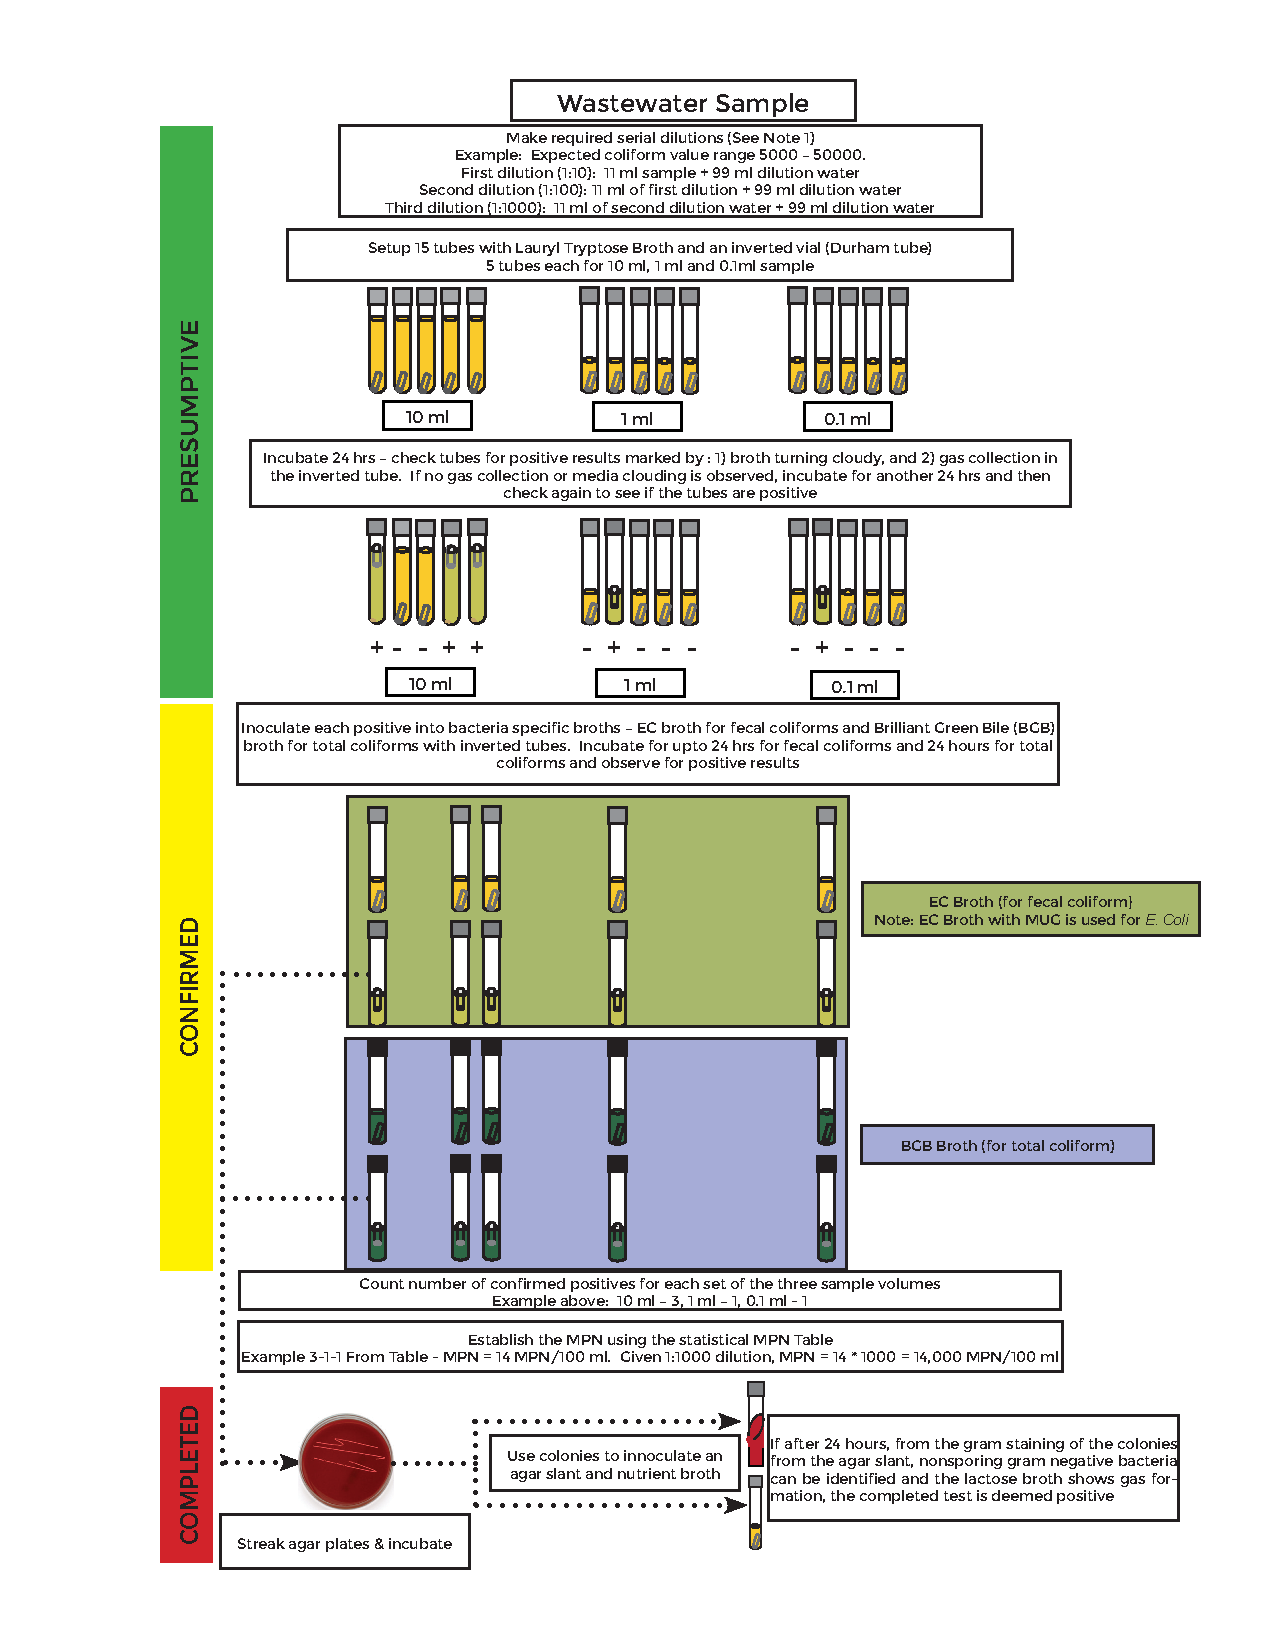
\includepdf[]{MTF.pdf}
%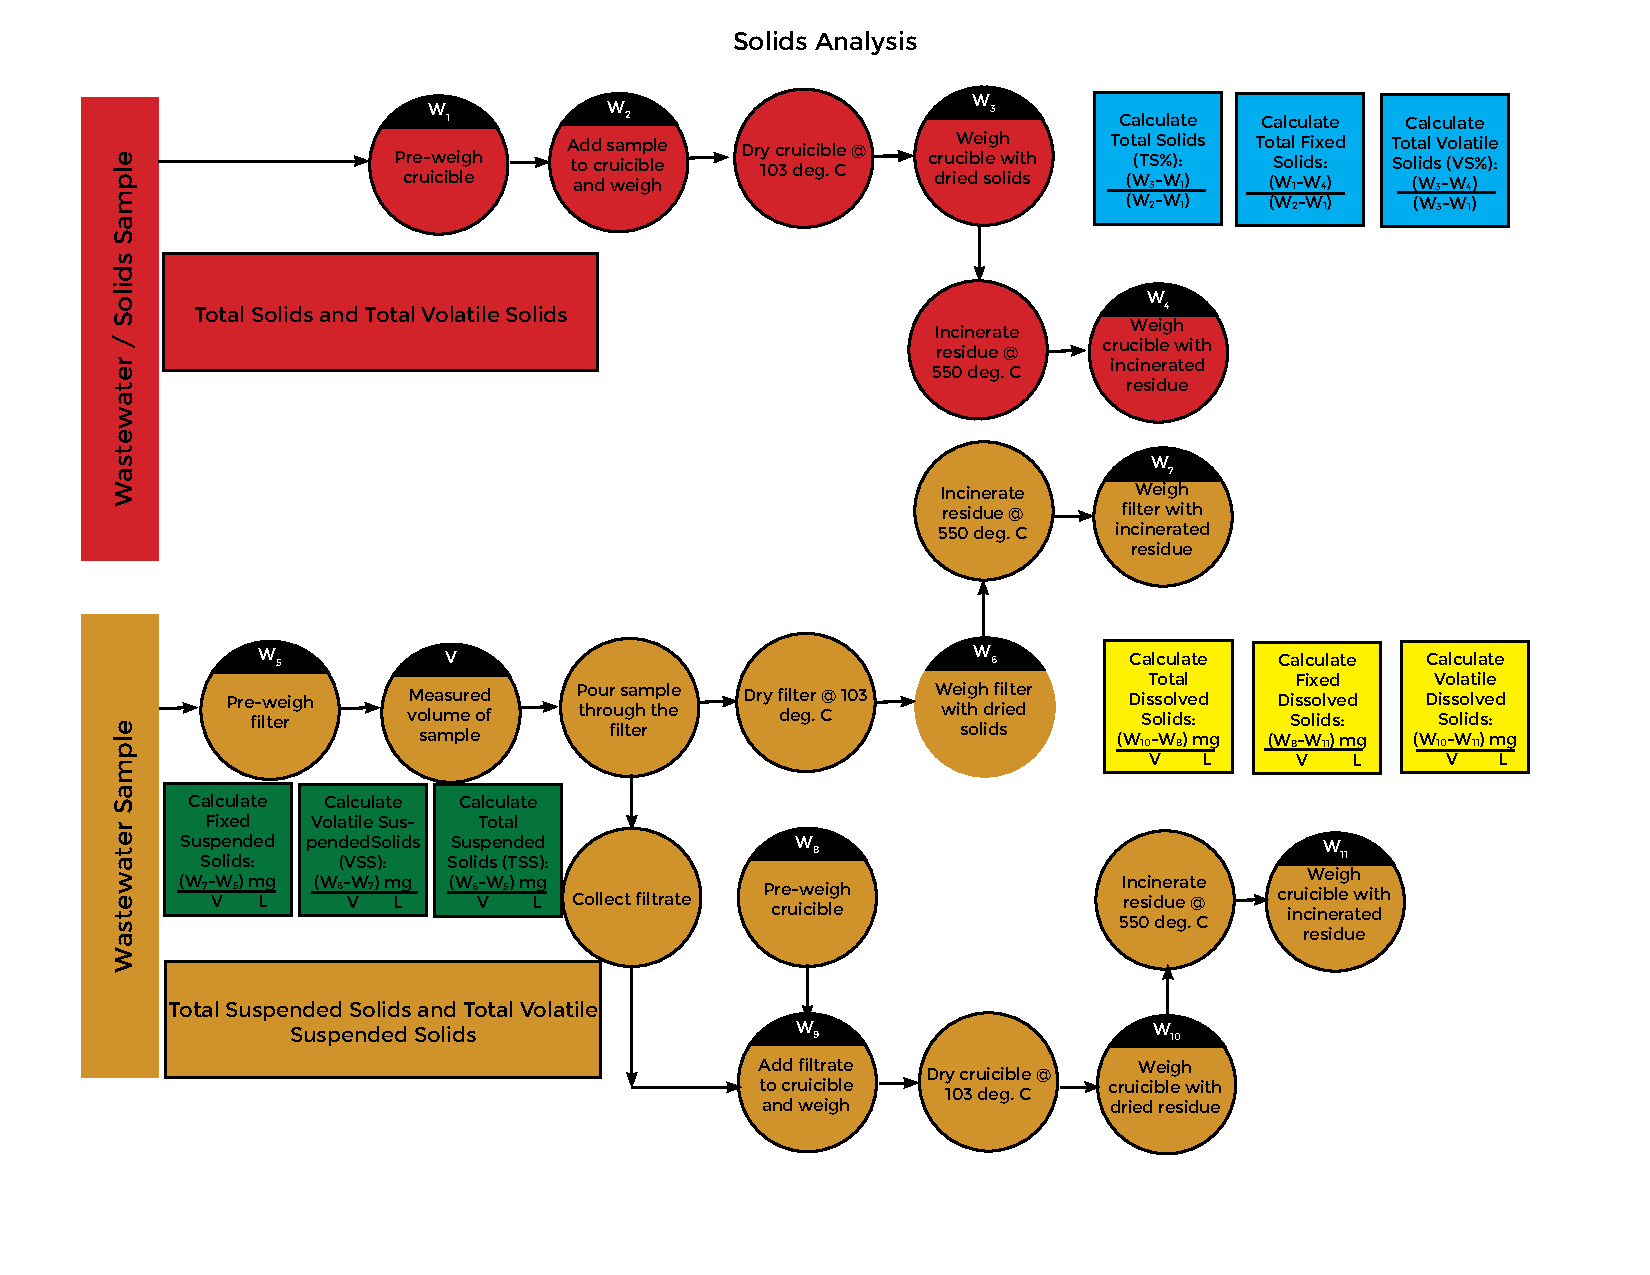
\includegraphics[scale=0.69]{LaboratorySolidsAnalysis4_01.pdf}
% \end{center}
% \end{landscape}
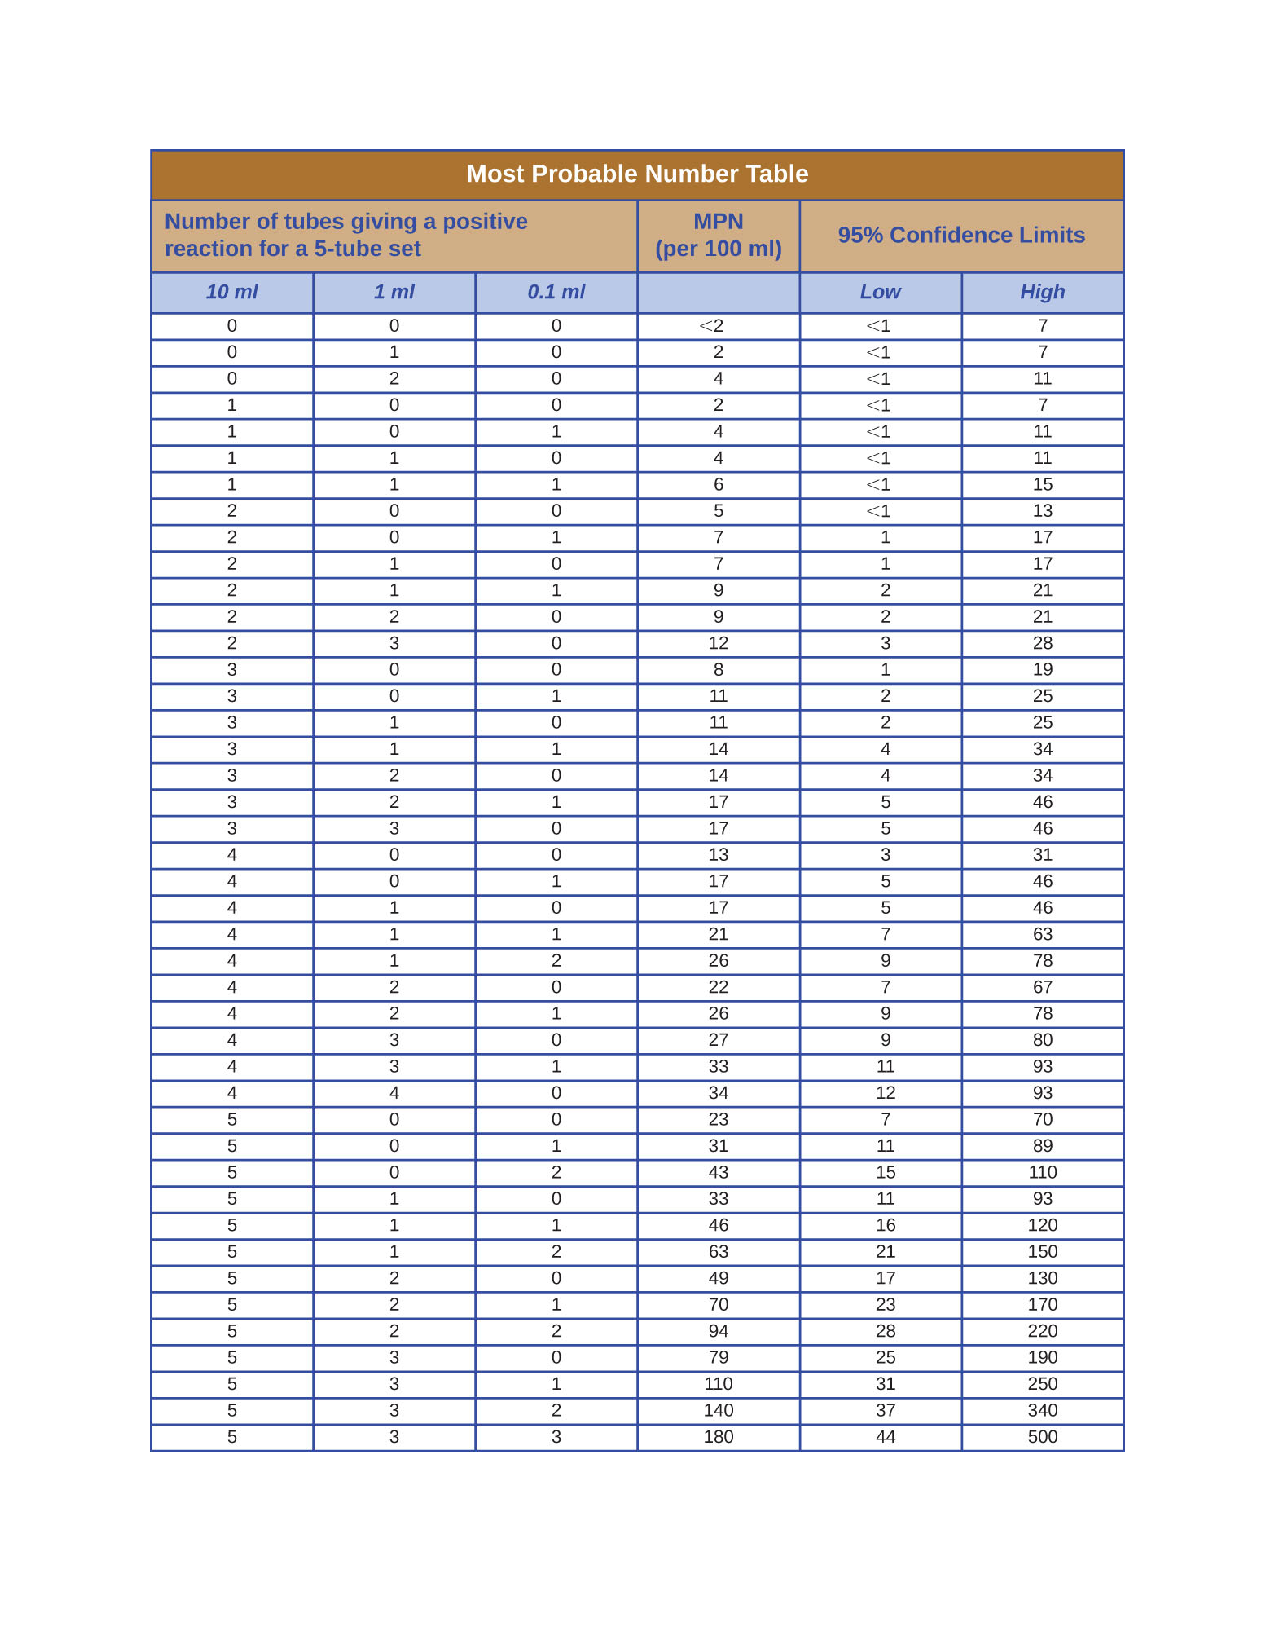
\includepdf[]{MTFTable.pdf}
\newpage
\subsection{The Membrane Filtration (MF) method}\index{The Membrane Filtration (MF) method}
This is a faster way to estimate bacterial populations in water.  In this method, an appropriate sample volume is passed through a membrane filter with a pore size small enough (0.45 micron) to retain the bacteria present. The filter is placed on an absorbent pad (in a petri dish) saturated with a culture medium that is selective for coliform growth. The petri dish containing the filter and pad is incubated, upside down, for 24 hours at the appropriate temperature. After incubation, the colonies that have grown are identified and counted using a low power microscope. A MUG medium is used for E- Coli.  If E. Coli is present, it will make the MUG fluorescent when viewed in UV light. 
\begin{center}
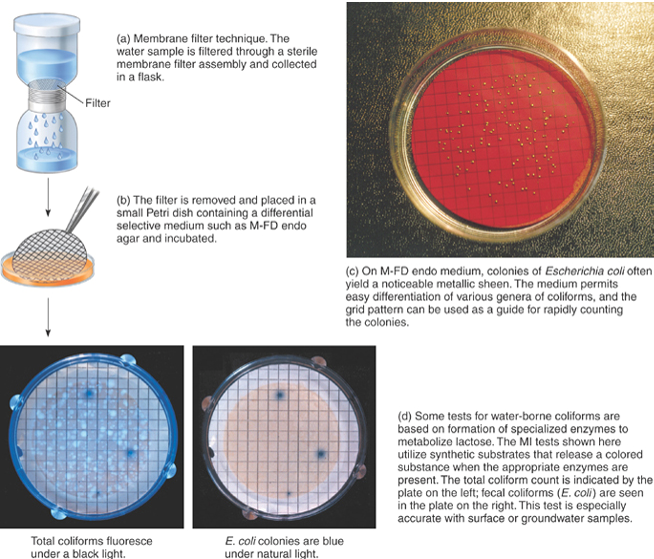
\includegraphics[scale=0.9]{LaboratoryMembraneFiltration}
\end{center}
\pagebreak

\subsection{Quanti-trays tests}\index{Quanti-trays tests}

This test used for the detection and quantification of specific microorganisms is being used increasingly mainly because it is a quicker test than the MTF.  Colilert and Enterolert are the quanti tray based tests for E. Coli and Enterococcus.  This method involve the use of specific enzymes and overcomes the drawbacks of the MTF which include false positives and negatives due to the more generic nature of the media used
\begin{center}
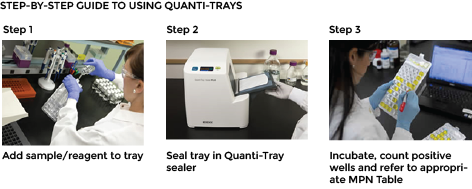
\includegraphics[scale=0.9]{LaboratoryQuantiTray}
\end{center}


